\documentclass[a4paper]{article}

\usepackage[UTF8]{ctex}
\usepackage[a4paper,margin=1in]{geometry}
\usepackage{graphicx}
\usepackage{float}
\usepackage{listings}
\usepackage{longtable}
\usepackage{booktabs}
\usepackage{hyperref}
\usepackage{fancyhdr}
\usepackage{lastpage}
\usepackage{color}
\usepackage{indentfirst}        % 首段缩进
\setlength{\parindent}{2em}     % 缩进2字符
\usepackage{zhnumber}           % 中文编号
\usepackage[dvipsnames]{xcolor}

%\newcommand{\college}{中山大学计算机学院}
\newcommand{\projname}{数据库系统原理实验|实验十二}
\newcommand{\reporttitle}{数据库并发事务实验}
\newcommand{\stuno}{23336179}
\newcommand{\authorname}{马福泉}
\newcommand{\major}{计算机科学与技术}
\newcommand{\adviser}{赖韩江}
\newcommand{\startdate}{2025年12月18日}
\newcommand{\labenddate}{2025年12月25日}
\newcommand{\labroom}{B202}

\pagestyle{fancy} % 使用 fancyhdr 风格
\fancyhf{}      % 清空默认的页眉页脚

% 设置页眉
\fancyhead[L]{\kaishu \projname}      % 左侧页眉显示项目名称
\fancyhead[C]{\kaishu \reporttitle}    % 中间页眉显示报告标题
\fancyhead[R]{\kaishu \authorname} % 右侧页眉显示作者姓名

% 设置页脚
\fancyfoot[C]{第 \thepage 页，共 \pageref{LastPage} 页} % 中间页脚显示页码

% 去除页眉页脚与正文之间的分隔线
\renewcommand{\headrulewidth}{0.4pt}
\renewcommand{\footrulewidth}{0pt}

% 设置文档背景颜色
\definecolor{mybgcolor}{RGB}{0, 0, 0} % 定义背景颜色
\definecolor{NavyBlue}{RGB}{0,0,128} % 添加颜色定义
% \pagecolor{mybgcolor} % 设置背景颜色

% listing 配置rust
% \lstdefinelanguage{Rust}{
%   keywords={fn, let, mut, struct, enum, impl, pub, use, mod, trait, where},
%   keywordstyle=\color{NavyBlue},
%   comment=[l]{//},
%   commentstyle=\color{gray},
% }
% \lstset{language=Rust}

\lstset{
  basicstyle=\ttfamily\small,
  keywordstyle=\color{NavyBlue},
  commentstyle=\color{gray},
  stringstyle=\color{red},
  showstringspaces=false,
  extendedchars=false, % 关键：不处理中文
  breaklines=true
}

\begin{document}

% 封面
\begin{titlepage}
    \centering
    
\includegraphics[width=10cm]{img/SYSULogo.png}

    \vspace{1em}
    %{\Large \college \par}
    \vspace{1em}
    {\Large \kaishu \projname \par}
    \vspace{3em}

    

    
    {\fontsize{40pt}{42pt}\kaishu \selectfont \boldmath \reporttitle\par}
    \vspace*{\fill}

    \begin{center}
    {\Large
    \makebox[5em][s]{学号}:\underline{\makebox[15em][c]{\kaishu \stuno}}\\[1em]
    \makebox[5em][s]{姓名}:\underline{\makebox[15em][c]{\kaishu \authorname}}\\[1em]
    \makebox[5em][s]{专业}:\underline{\makebox[15em][c]{\kaishu \major}}\\[1em]
    \makebox[5em][s]{课程教师}:\underline{\makebox[15em][c]{\kaishu \adviser}}\\[1em]
    \makebox[5em][s]{起始日期}:\underline{\makebox[15em][c]{\kaishu \startdate}}\\[1em]
    \makebox[5em][s]{结束日期}:\underline{\makebox[15em][c]{\kaishu \labenddate}}\\[1em]
    \makebox[5em][s]{实验地点}:\underline{\makebox[15em][c]{\kaishu \labroom}}
    }
    \end{center}

    \vspace*{\fill}
\end{titlepage}

% 目录
\tableofcontents
\newpage


\section{实验概述}

\subsection{实验目的}
熟悉数据库并发事务的相关操作实验。

\subsection{实验内容}
1. 创建一个事务：在record表中插入一条新记录，同时修改book表中的interview\_times为interview\_times+1，以保证数据的一致性。（参考实验教材4.1）

2. 编写事务程序，用于更新book表中的SQL Server 2012宝典的信息，观察其事务过程中锁的获得与释放情况，以及锁定资源的类型。（参考4.2）

3. 编写事务程序，对book表进行实验，设置相应的隔离级别，模拟实现读脏数据、不可重复读以及可重复读。（参考4.3）

4. 编写事务程序，对book表进行实验，设计实验制造事务之间的死锁。（参考4.4）
\section{实验报告}

\subsection{创建事务并保证数据一致性}
\textbf{实验目的：} 验证事务的原子性（Atomicity）。通过编写一个事务，模拟借书操作：在 record 表中插入一条借阅记录，同时将 book 表中对应书籍的“借阅次数”加1。

\textbf{实验代码：}
\begin{lstlisting}[language=SQL]
BEGIN TRANSACTION;
-- 1. 插入借阅记录
INSERT INTO dbo.record (reader_id, book_id, borrow_date, return_date, notes)
VALUES ('r0004', 'b0001', GETDATE(), DATEADD(day, 30, GETDATE()), '一致性测试');
-- 2. 更新书籍借阅次数 (interviews_times)
UPDATE dbo.book
SET interviews_times = interviews_times + 1
WHERE book_id = 'b0001';
COMMIT TRANSACTION;
-- 验证数据
SELECT * FROM dbo.record WHERE book_id = 'b0001';
SELECT book_id, interviews_times FROM dbo.book WHERE book_id = 'b0001';
\end{lstlisting}

\textbf{实验结果：}
\begin{figure}[H]
    \centering
    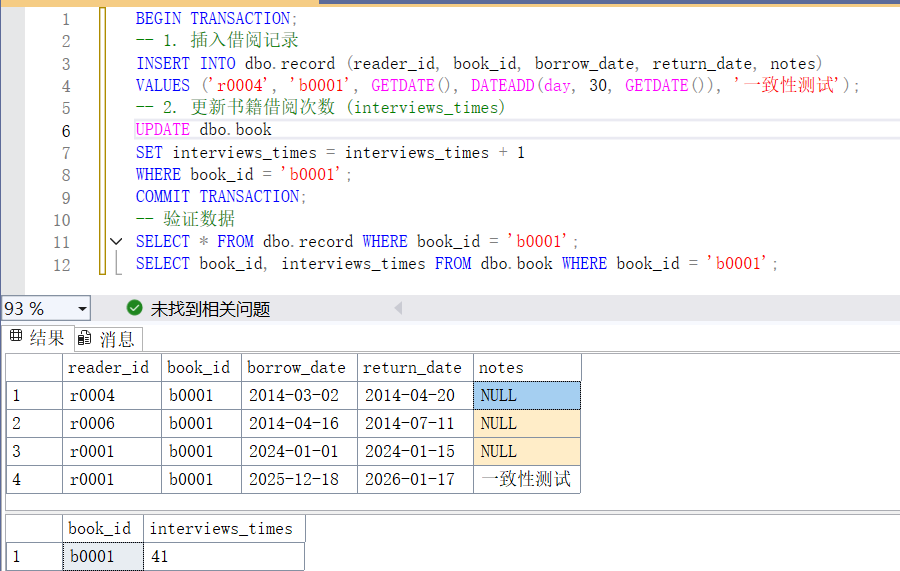
\includegraphics[width=0.7\textwidth]{img/step1_consistency.png}
    \caption{数据一致性验证结果}
\end{figure}

\textbf{结果分析：}如上图所示，查询结果显示 record 表成功插入了新记录，同时 book 表的 interviews\_times 字段数值增加了 1。说明事务内的两个操作要么全部成功，保证了数据的一致性。

\subsection{观察锁的获得与释放}
\textbf{实验目的：} 观察事务在执行过程中对资源锁定的情况。

\textbf{实验代码：}
\begin{lstlisting}[language=SQL]
BEGIN TRANSACTION;
-- 更新操作，但在提交前暂停
UPDATE dbo.book SET book_price = 120.00 WHERE book_name = 'SQL Server 2012宝典';

-- 查询当前会话持有的锁
SELECT resource_type, request_mode, resource_description, request_status 
FROM sys.dm_tran_locks
WHERE request_session_id = @@SPID;
COMMIT TRANSACTION;
\end{lstlisting}

\textbf{实验结果：}
\begin{figure}[H]
    \centering
    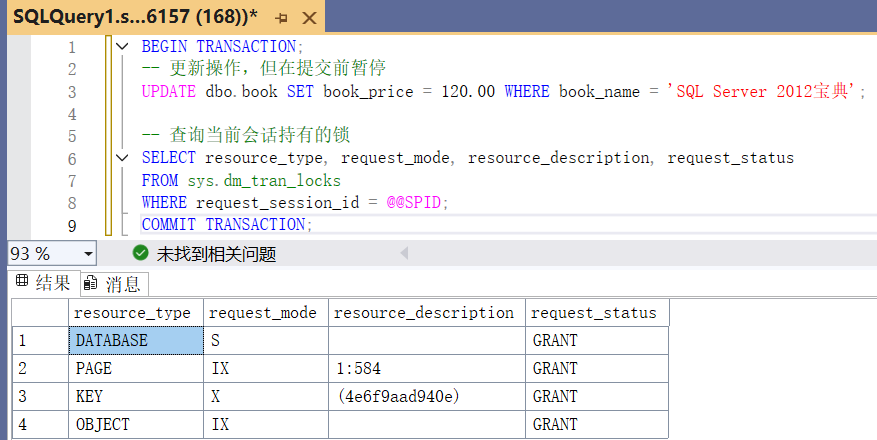
\includegraphics[width=0.7\textwidth]{img/step2_locks.png}
    \caption{锁持有情况查询结果}
\end{figure}

\textbf{结果分析：}如上图所示，在事务提交之前，系统视图显示当前会话对 book 表的相关资源持有了 X 锁（排他锁），表明在事务结束前，该资源被当前事务独占，其他事务无法修改。

\subsection{事务隔离级别模拟}

\subsubsection{脏读 (Read Uncommitted) 模拟与回滚验证}
\textbf{实验目的：} 验证在 READ UNCOMMITTED 隔离级别下，事务可以读取到其他事务未提交的修改。

\textbf{实验代码：}
\begin{lstlisting}[language=SQL]
-- 窗口 A：执行更新但不提交
BEGIN TRAN;
UPDATE dbo.book SET interviews_times = 999 WHERE book_id = 'b0001';

-- 窗口 B：设置隔离级别并查询
SET TRANSACTION ISOLATION LEVEL READ UNCOMMITTED;
SELECT interviews_times FROM dbo.book WHERE book_id = 'b0001';

-- 回滚操作：窗口 A 执行
ROLLBACK;
\end{lstlisting}

\textbf{实验结果：}
\begin{figure}[H]
    \centering
    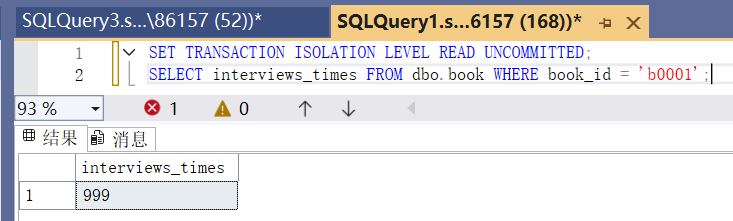
\includegraphics[width=0.7\textwidth]{img/1.png}
    \caption{窗口 B 读到了窗口 A 尚未提交的脏数据 999}
\end{figure}
\begin{figure}[H]
    \centering
    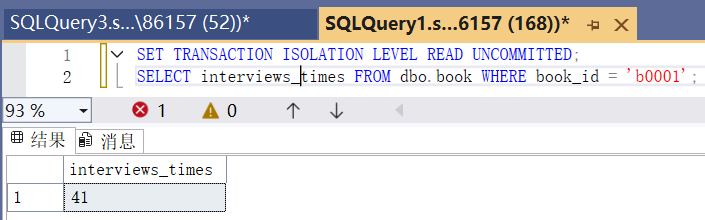
\includegraphics[width=0.7\textwidth]{img/2.png}
    \caption{窗口 A 回滚后，窗口 B 再次查询发现数据恢复为 41}
\end{figure}

\textbf{结果分析：} 在 READ UNCOMMITTED 级别下，数据库允许“脏读”。实验显示窗口 B 读取到了窗口 A 未提交的中间值。当窗口 A 回滚后，数据恢复原状，证明了脏读现象的存在。

\subsubsection{不可重复读 (Read Committed) 验证}
\textbf{实验目的：} 验证在 READ COMMITTED 级别下，同一事务内两次读取之间由于其他事务的提交导致结果不一致。

\textbf{实验代码：}
\begin{lstlisting}[language=SQL]
-- 窗口 A：开启事务并进行第一次读取
SET TRANSACTION ISOLATION LEVEL READ COMMITTED;
BEGIN TRAN;
SELECT interviews_times FROM dbo.book WHERE book_id = 'b0001';

-- 窗口 B：修改数据并提交
UPDATE dbo.book SET interviews_times = 50 WHERE book_id = 'b0001';
COMMIT;

-- 窗口 A：再次执行查询
SELECT interviews_times FROM dbo.book WHERE book_id = 'b0001';
COMMIT;
\end{lstlisting}

\textbf{实验结果：}
\begin{figure}[H]
    \centering
    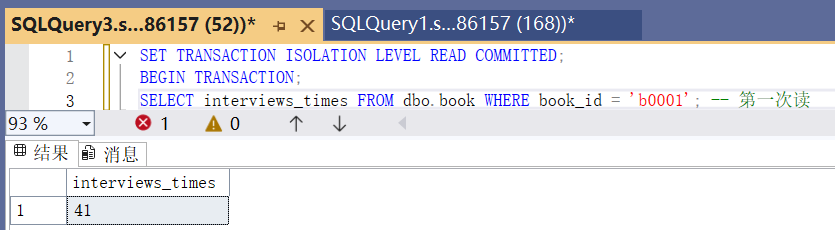
\includegraphics[width=0.7\textwidth]{img/3.png}
    \caption{窗口 A 第一次读取结果为 41}
\end{figure}
\begin{figure}[H]
    \centering
    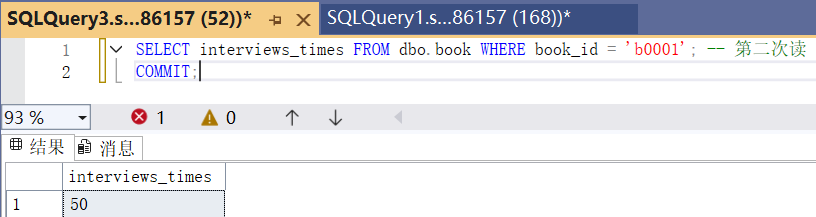
\includegraphics[width=0.7\textwidth]{img/4.png}
    \caption{窗口 B 提交修改后，窗口 A 第二次读取结果变为了 50}
\end{figure}

\textbf{结果分析：} READ COMMITTED 级别避免了脏读，但允许不可重复读。窗口 A 在同一事务内的两次读取结果不同，是因为窗口 B 在两次读取之间提交了更新。

\subsubsection{可重复读 (Repeatable Read) 与锁阻塞验证}
\textbf{实验目的：} 验证 REPEATABLE READ 通过锁定读取的行，确保在事务结束前该行数据不会被其他事务修改。

\textbf{实验代码：}
\begin{lstlisting}[language=SQL]
-- 窗口 A：设置隔离级别并开启事务
SET TRANSACTION ISOLATION LEVEL REPEATABLE READ;
BEGIN TRAN;
SELECT interviews_times FROM dbo.book WHERE book_id = 'b0001';

-- 窗口 B：尝试更新同一行数据
UPDATE dbo.book SET interviews_times = 55 WHERE book_id = 'b0001';

-- 窗口 A：再次查询并提交
SELECT interviews_times FROM dbo.book WHERE book_id = 'b0001';
COMMIT;
\end{lstlisting}

\textbf{实验结果：}
\begin{figure}[H]
    \centering
    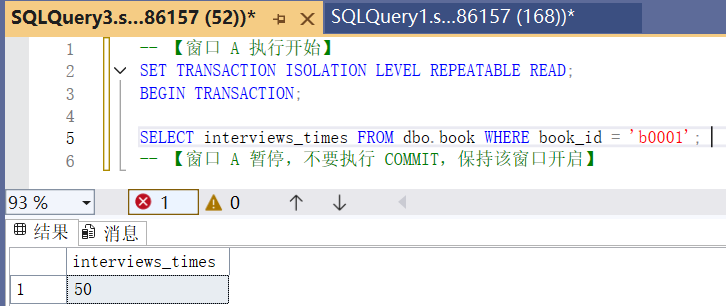
\includegraphics[width=0.7\textwidth]{img/5.png}
    \caption{窗口 A 启动事务并读取结果为 50}
\end{figure}
\begin{figure}[H]
    \centering
    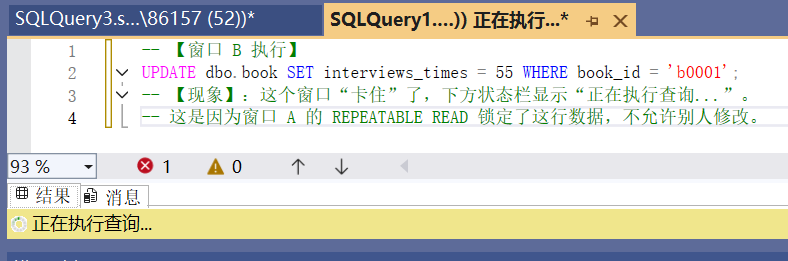
\includegraphics[width=0.7\textwidth]{img/6.png}
    \caption{窗口 B 执行更新语句时发生阻塞，下方状态栏显示“正在执行查询”，证明窗口 A 持有的 S 锁阻止了窗口 B 获取 X 锁}
\end{figure}
\begin{figure}[H]
    \centering
    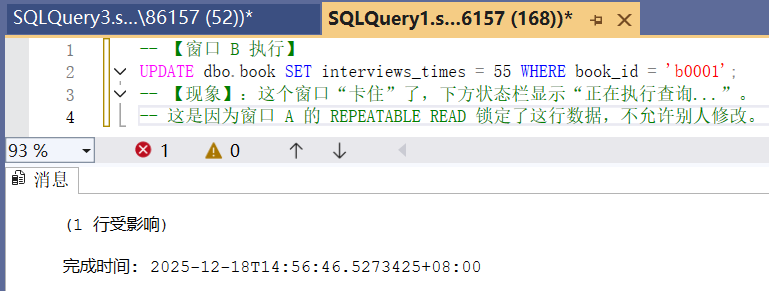
\includegraphics[width=0.7\textwidth]{img/7.png}
    \caption{窗口 B 在窗口 A commit 后结束阻塞}
\end{figure}
\begin{figure}[H]
    \centering
    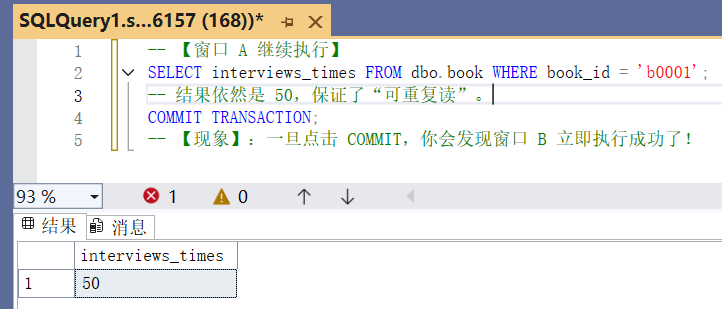
\includegraphics[width=0.7\textwidth]{img/8.png}
    \caption{窗口 A 再次查询，结果依然是 50，提交事务后窗口 B 才成功执行}
\end{figure}

\textbf{结果分析：} 在 REPEATABLE READ 级别下，窗口 A 对读取的行持有共享锁（S 锁）直到事务结束。这导致窗口 B 的更新操作（需要排他锁 X 锁）被阻塞。只有当窗口 A 提交事务释放锁后，窗口 B 才能继续执行，从而确保了窗口 A 在事务期间读取数据的一致性。

\subsection{实验四：模拟并制造事务死锁 (Deadlock)}
\subsubsection{实验步骤}
\begin{enumerate}
    \item \textbf{准备阶段：} 打开两个 SSMS 查询窗口，均连接至 \texttt{JY} 数据库，并并排显示以便观察时序。
    \item \textbf{事务构建：} 在两个窗口中分别编写逻辑相反的事务程序。事务 A 先锁书籍 \texttt{b0001} 再请求 \texttt{b0002}；事务 B 先锁 \texttt{b0002} 再请求 \texttt{b0001}。
    \item \textbf{并发执行：} 几乎同时启动两个窗口的脚本，通过 \texttt{WAITFOR DELAY} 确保两个事务都能先获取到各自的第一把锁，从而形成循环等待。
\end{enumerate}

\subsubsection{实验代码}
\begin{minipage}[t]{0.45\textwidth}
\begin{lstlisting}[caption={窗口 1：事务 A}]
-- 事务 A：先锁 b0001，再请求 b0002
USE JY; GO
PRINT '事务A开始...';
BEGIN TRANSACTION;
  UPDATE book 
  SET book_price = book_price + 1 
  WHERE book_id = 'b0001';
  
  PRINT '事务A已锁b0001, 等待5秒...';
  WAITFOR DELAY '00:00:05';
  
  UPDATE book 
  SET book_price = book_price + 1 
  WHERE book_id = 'b0002';
COMMIT TRANSACTION;
\end{lstlisting}
\end{minipage}
\hfill
\begin{minipage}[t]{0.45\textwidth}
\begin{lstlisting}[caption={窗口 2：事务 B}]
-- 事务 B：先锁 b0002，再请求 b0001
USE JY; GO
PRINT '事务B开始...';
BEGIN TRANSACTION;
  UPDATE book 
  SET book_price = book_price - 1 
  WHERE book_id = 'b0002';
  
  PRINT '事务B已锁b0002, 等待5秒...';
  WAITFOR DELAY '00:00:05';
  
  UPDATE book 
  SET book_price = book_price - 1 
  WHERE book_id = 'b0001';
COMMIT TRANSACTION;
\end{lstlisting}
\end{minipage}

\subsubsection{实验结果与现象分析}
\begin{figure}[H]
    \centering
    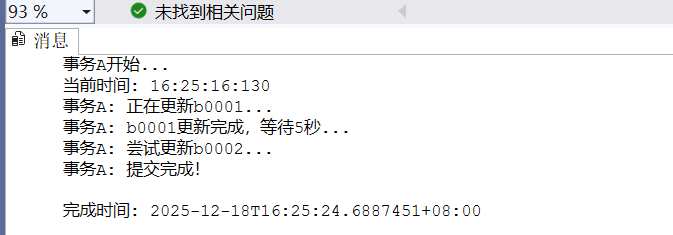
\includegraphics[width=0.85\textwidth]{img/A_success.png}
    \caption{事务 A 执行成功：作为死锁竞争中的幸存者正常提交}
\end{figure}

\begin{figure}[H]
    \centering
    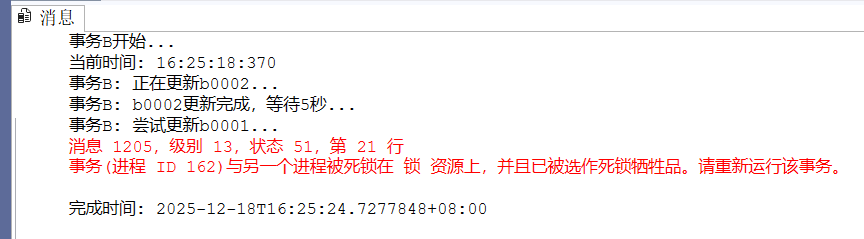
\includegraphics[width=0.85\textwidth]{img/B_fail.png}
    \caption{事务 B 执行失败：触发 1205 错误，被选作死锁牺牲品}
\end{figure}

\textbf{结果判定：} 
实验成功触发死锁。如图所示，事务 B 在尝试更新 \texttt{b0001} 时，系统检测到循环等待，报错：\textit{“消息 1205, 级别 13, 事务（进程 ID 162）与另一个进程被死锁在锁资源上，并且已被选作死锁牺牲品”}。此时事务 B 自动回滚，释放锁资源，使得事务 A 能够完成后续更新并成功提交。

% --- 实验总结部分 ---
\section{实验总结与问题分析}

\subsection{主要收获}
通过本次实验，我系统地理解了事务的 ACID 特性以及并发控制的重要性。我掌握了如何通过设置 \texttt{TRANSACTION ISOLATION LEVEL} 来控制并发副作用，并学会了利用系统动态管理视图监控锁资源。

\subsection{困难与解决方法 (Troubleshooting)}
在实验过程中，我遇到了以下代表性的技术问题，并逐一进行了排查与解决：

\begin{enumerate}
    \item \textbf{非预期的事务阻塞 (Blocking)：}
    在模拟死锁之前，我发现即使只执行一条 \texttt{UPDATE} 语句，窗口也会长时间处于“正在执行查询”状态（见图 \texttt{bug.png}）。
    
    \begin{figure}[H]
        \centering
        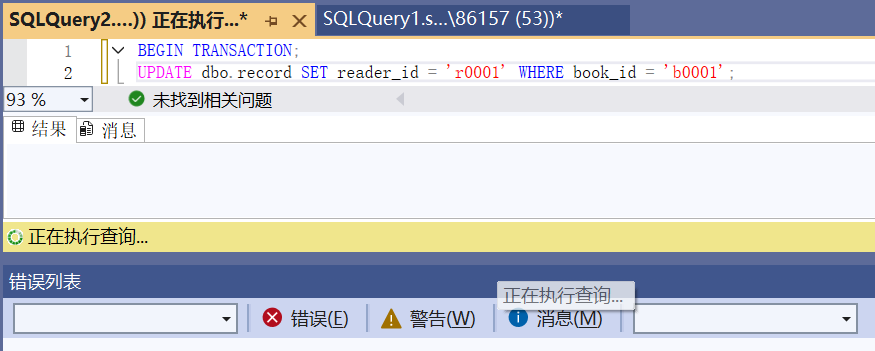
\includegraphics[width=0.7\textwidth]{img/bug.png}
        \caption{非预期阻塞现象：窗口处于持续挂起状态}
    \end{figure}
    
    \item \textbf{死锁残留与后台进程监控：}
    通过查询 \texttt{sys.dm\_tran\_locks} 视图（见图 \texttt{bug2.png}），我发现会话 53 持有了 \texttt{KEY} 的排他锁 (\texttt{X})。这说明之前的实验事务未正常回滚或提交，导致资源被永久锁定。
    
    \begin{figure}[H]
        \centering
        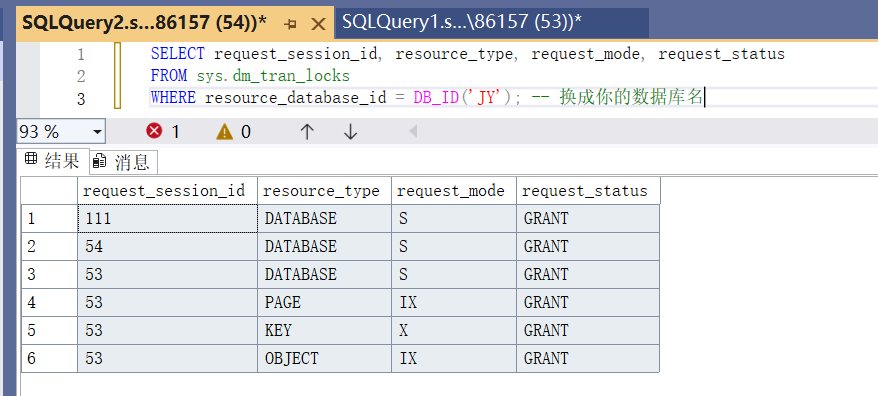
\includegraphics[width=0.8\textwidth]{img/bug2.png}
        \caption{利用 DMV 视图排查锁资源：Session 53 持有排他锁}
    \end{figure}
    
    \item \textbf{约束冲突问题：}
    在更新 \texttt{record} 表时，曾因修改外键字段导致 \texttt{547} 约束冲突，或修改主键字段导致 \texttt{2627} 冲突。
\end{enumerate}

\textbf{最终解决方法：} 
针对上述问题，我采取了以下措施：首先通过执行 \texttt{ROLLBACK} 或 \texttt{KILL} 命令强制关闭残留的僵尸进程；其次，在死锁实验中将更新对象统一为非约束字段（如 \texttt{book\_price}），避开了业务逻辑干扰。这些调试过程加深了我对数据库排他锁 (X Lock) 与意向排他锁 (IX Lock) 互斥关系的理解。

\end{document}
